\documentclass{article}[12pt]
\renewcommand{\baselinestretch}{1.5}

\usepackage[parfill]{parskip}
\usepackage[affil-it]{authblk}
\usepackage[space]{grffile}

\usepackage[a4paper]{geometry}
\geometry{verbose}
\usepackage{float}
\usepackage{graphicx}
\usepackage{setspace}
\usepackage{caption}

\usepackage[utf8]{inputenc}
\usepackage[english]{babel}

\usepackage{xcolor}
\definecolor{Green}{rgb}{0.0, 0.5, 0.0}

\usepackage{latexsym,textcomp,longtable,tabulary}
\usepackage{booktabs,array,multirow,braket}
\usepackage{amsfonts,amsmath,amssymb,mathbbol,calc}
\usepackage{subfigure,color,blindtext,enumitem,siunitx}

\usepackage{mathtools}
\usepackage{url,hyperref,etoolbox}
\numberwithin{equation}{section}
\hypersetup{colorlinks=false,pdfborder={0 0 0}}

%+figure layout options
\restylefloat{figure}
\setlist{leftmargin=*,before=\setlength{\rightmargin}{\leftmargin}}
%-figure layout options

\providecommand\citet{\cite}
\providecommand\citep{\cite}
\providecommand\citealt{\cite}

\setlength{\parskip}{1em}
\makeatletter
\makeatother


\newif\iflatexml\latexmlfalse
\providecommand{\tightlist}{\setlength{\itemsep}{0pt}\setlength{\parskip}{0pt}}%
\AtBeginDocument{\DeclareGraphicsExtensions{.pdf,.PDF,.eps,.EPS,.png,.PNG,.tif,.TIF,.jpg,.JPG,.jpeg,.JPEG}}
\begin{document}

\title{
Field Theory Methods \\
in Reaction-Diffusion Systems
}

\author{Gregory Szep}
\affil{King's College London}
\date{\today}
\maketitle
\vspace{-25pt}
\section{Dynamical Systems Approach} \vspace{-10pt}
In this section we will set the scene for chemical reaction systems and their
methods of analysis of steady state and network perspectives. Dynamical
methods makes use of field flow, linear stability and bifurcation analysis.
\subsection{Reaction Kinetics} \vspace{-10pt}
Consider $N$ particles of $S$ species in a finite volume $\Omega$. These particles
can undergo $R$ possible reactions when they meet within the volume. Suppose the
timescales of equilibration with respect to volume and temperature are much faster
than that of species number equilibration. This means that non-reactive collisions
occur more frequently than collisions that trigger any of the $R$ reactions. This
is the essence of the \textit{well-mixed} approximation \cite{Gillespie1992}.

This suggests that at any time $t$ we may ignore spatial inhomogeneities and pin
down the state of the system by a vector of species populations $s(t)\in\mathbb{N}^S$.
All possible reactions in the mixture are encoded into a stoichiometric matrix
$\mathbf{\Gamma}\in\mathbb{Z}^{S\times R}$ whos columns $\mathbf{\Gamma}[r]\in\mathbb{Z}^{S}$
represent the population change vector for a given reaction $r$. Each reaction
has a propensity $\omega(r|s)\in[0,\infty)$ defined though transition
probabilities for an infinitesimal time interval given population $s$;
\begin{align}
	\omega(r|s)\mathrm{d}t := \mathbb{P}(s+\mathbf{\Gamma}[r],t+\mathrm{d}t|s,t)
	\label{eq:fundamentalpremise}
\end{align}
Suppose $\sigma[r]\mathrm{d}t$ gives the probability that the reaction $r$
will occur within the time interval $\mathrm{d}t$ independent of population
$s$. The constant $\sigma[r]$ could be in principle calculated from the
microscopic physics of the reaction. In quantum mechamics this would involve
calculating the wavefunction overlap or transition rates between initial and
final configurations.

The propensity is proportional this rate, up to combinatoric multiplicity
taking into account the species population $s$. A reaction $r$ chooses $g[i,r]$
particles for each reactant species $i$ from the $well-mixed$ solution containing
$s[i]$ particles. Thus the multiplicity is simply given by a binomial coefficient
per species. This results in a propensity that is polynomial in the components
$s[i]$, where the highest power term gives us the \textit{order} of the reaction.
\begin{align}
	\omega(r|s)=
	\sigma[r]
		\prod_{i=1}^S{s[i] \choose g[i,r]}
	\label{eq:propensity}
\end{align}
For reactions involving distinguishable particle species, all
components $ g[i,r]\in\{ 0,1\}$ and simplifies the combinatoric term to a
product of all reactant populations.
\begin{align}
	g[i,r]\in\{ 0,1\}\quad\forall i,r\quad\implies\quad
	\omega(r|s)=
	\sigma[r]
	\prod_{i=1}^S s[i]^{g[i,r]}
	\label{eq:simplifiedpropensity}
\end{align}
\subsubsection{Chemical Master Equation}\vspace{-10pt}
By applying the laws of probability and taking the $\mathrm{d}t\rightarrow 0$
one can derive --- see Appendix \ref{a:cme} for details --- a time-evolution equation
$\mathbb{P}(s,t)$ involving the definition \eqref{eq:fundamentalpremise} which
has become known as the Chemical Master Equation \cite{Gillespie1992,Gillespie2007}.
Note here the complexity lies within the nonlinear state dependence in the propensity
$\omega(r|s)$. Were it not for this, we could solve this equation using
spectral methods.
\begin{align}
	\partial_t\mathbb{P}(s,t) &=
	\sum_{r=1}^R
	\omega(r|s-\mathbf{\Gamma}[r])\mathbb{P}(s-\mathbf{\Gamma}[r],t)-\omega(r|s)\mathbb{P}(s,t)
	\label{eq:cme}
\end{align}
Multiplying the Chemical Master Equation \eqref{eq:cme} by $s$ and summing over all $s$
obtains a system of differential equations for the first moment
$\left\langle s \right\rangle$ in terms of vectorised propensity
$\omega(s|\mathbf{\Gamma})\in[0,\infty)^R$ which couples to higher order moments,
unfolding an infinte heirarchy.
\begin{align}
	\partial_t
	\left\langle s \right\rangle &=
	\mathbf{\Gamma} \big\langle \omega(s|\mathbf{\Gamma}) \big\rangle
	\label{eq:momentheirarchy}
\end{align}
\subsubsection{Reaction Equation}\vspace{-10pt}
The mean field approximation factorises higher order moments, implying
$\big\langle f(s) \big\rangle=f(\langle s\rangle)$ for any nonlinear
function $f$. This is equivalent to neglecting fluctuations in the
$N,\Omega\rightarrow\infty$
thermodynamic limit, and it is here where the mass-action assumption
becomes manifest \cite{Gillespie2007}.

This closes the infinite heirarchy
\eqref{eq:momentheirarchy} yielding a nonlinear set of coupled ordinary
differential equations for a continuous vector field $\psi(t)\in[0,\infty)^S$.
These have come to be known as the Reaction Rate Equations, and are
typical for modelling processes in systems biology.
\begin{align}
	\partial_t
	\psi &=
	\mathbf{\Gamma}\omega(\psi|\mathbf{\Gamma})
	\label{eq:reaction}
\end{align}
\vspace{-40pt}
\subsubsection{Bifurcation Analysis}\vspace{-15pt}
In the mean field approximation \eqref{eq:reaction} we may investigate the
steady state $\partial_t\psi=0$. This gives rise to a set of $S$ polynomial
equations in the components $\psi[s]\in[0,\infty)$ of steady state $\psi^*$
These define $S-1$ dimensional nullcline hypersurfaces embedded in $S$
dimensional state space.
\begin{align}
	\sum_{r=1}^R\Gamma[s',r]\sigma[r]
		\prod_{s=1}^S{\psi[s] \choose g[s,r]}
		\bigg|_{\psi=\psi^*}
		=0\qquad\forall s'=1,2,\dots,S
	\label{eq:steadystate}
\end{align}
\vspace{-20pt}
\begin{figure}[H]
\centering{}
\captionsetup{justification=centering}
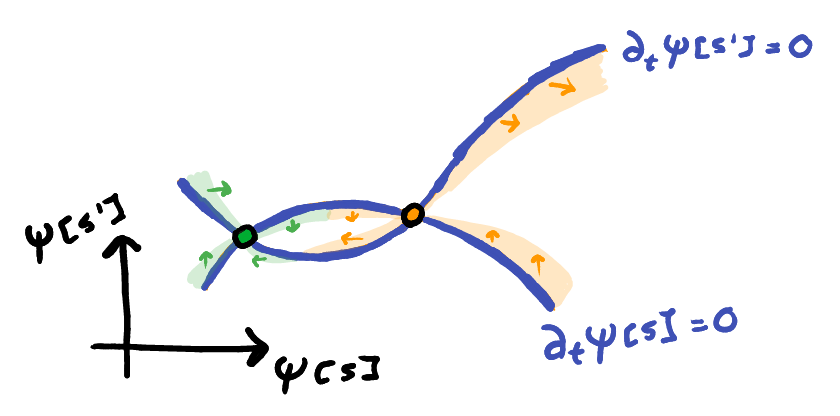
\includegraphics[scale=0.35]{figures/nullclines}
\caption{Schematic of two nullclines with their orthogonal local\\ field flows intersecting
at \textcolor{Green}{stable} and \textcolor{orange}{unstable} fixed points $\psi^*$}
\label{fig:nullclines}
\end{figure}
Nullclines determine local direction of evolution of the system. On a given
nullcine $\partial_t\psi[s]=0$ the flow of the field must be orthogonal to
the direction of $\psi[s]$. At intersections between two nullclines, the flow
must be orthogonal to the plane defined by two axes. At the interections between
all nullcines we may find the fixed points $\psi^*$ as shown in Figure \ref{fig:nullclines}.

Classification of fixed points $\psi^*$ is done by linearising the equation of motion
\eqref{eq:reaction} with respect to field perturbation $\varepsilon(t)$ in their vicinity
and determining the eigenvalues of the resultant $S\times S$ Jacobian $\mathbf{J}(\psi)$
evaluated at each fixed point $\psi^*$.
\begin{align}
	\varepsilon(t) \sim
	\mathbb{e}^{\mathbf{J}(\psi)|_{\psi=\psi^*}t}\qquad\qquad\qquad\qquad\qquad\qquad
	\\
	\quad\text{where}\quad
	\mathrm{J}[i,j]=
	\sum_{r=1}^R
	\sigma[r]
\bigg(H(\psi[i])-H(\psi[i]-g[i,r])\bigg)
	\Gamma[j,r]
		\prod_{s=1}^S{\psi[s] \choose g[s,r]}
	\\
	H(x)=\int_0^1\frac{1-t^x}{1-t}\mathrm{d}t\quad
	\text{are generalised Harmonic Numbers}\qquad
	\label{eq:linearstability}
\end{align}
For reactions involving one or two distinguishable particles as
in \eqref{eq:simplifiedpropensity} the nullcines become hyperplanes and the Jacobian
simplifies. We can see that both the reaction topology given by stoichiometric
coefficients $\Gamma[i,j]$ and the reaction rates $\sigma[r]$ contribute to
rotating and shifting the hyperplanes and determining the location and stability
of their intersections.
\begin{align}
	\mathrm{J}[i,j]=
	\sum_{r=1}^R
		\sigma[r]|\Gamma[i,r]|\Gamma[j,r]
		\prod_{\,s\neq i}
		\psi[s]^{g[i,r]}
		\qquad g[i,r]\in\{0,1\} \quad\forall i,r
	\label{eq:simplifiedjacobian}
\end{align}
The sign of eigenvalues $\lambda$ of Jacobian $\mathbf{J}$ determine whether a fixed point
is stable $\lambda<0$ or unstable $\lambda>0$. As an illustrative example we can characterise
fixed points given an arbitrary two dimensional Jacobian. Figure \ref{fig:stability} reveals
the regions of stability and phase space flows.
\begin{figure}[H]
\centering{}
\captionsetup{justification=centering}
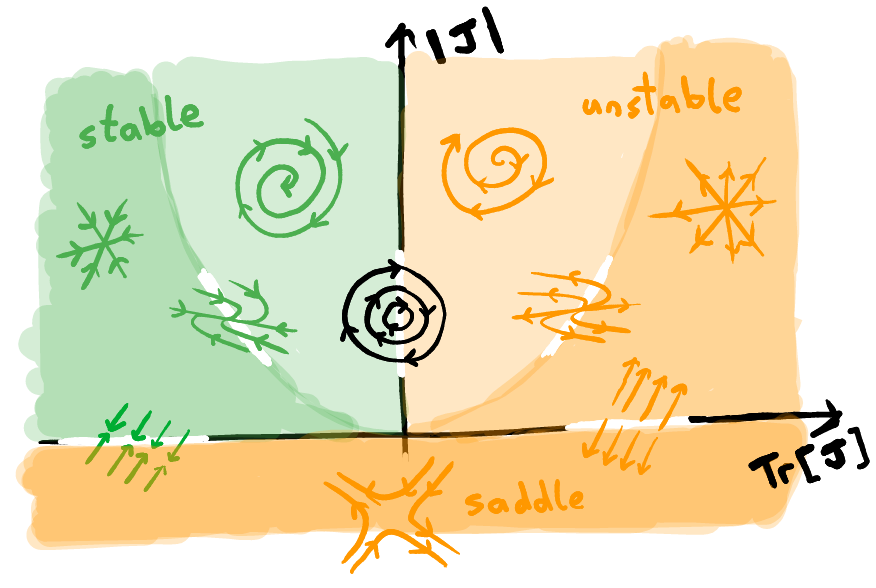
\includegraphics[scale=0.35]{figures/stability}
\caption{Classification of \textcolor{Green}{stable} and \textcolor{orange}{unstable}
fixed points for a general \\two dimensional Jacobian in terms of trace $\mathrm{Tr}[\mathbf{J}]$ and
determinant $|\mathbf{J}|$}
\label{fig:stability}
\end{figure}
Varying the continous parameters $\sigma[r]$ moves the nullcines and may result in
the creation or annihilation of fixed points of different classes. While an indiviual
fixed point may change location and local phase space flow, it cannot change class
without involving another fixed point.

These are called bifurcations and also fall into various catagories.
Figure \ref{fig:bifurcations} illustrates some of the possible one parameter
supercritical bifurcations; subcritical cases are obtained by permuting
stabilities of fixed points. Note the hysterisis loop in the saddle-node
bifurcation.
\begin{figure}[H]
\centering{}
\captionsetup{justification=centering}
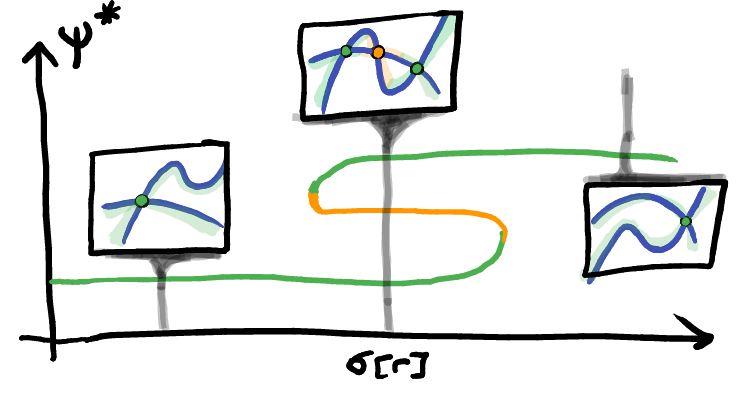
\includegraphics[scale=0.35]{figures/saddlenode}
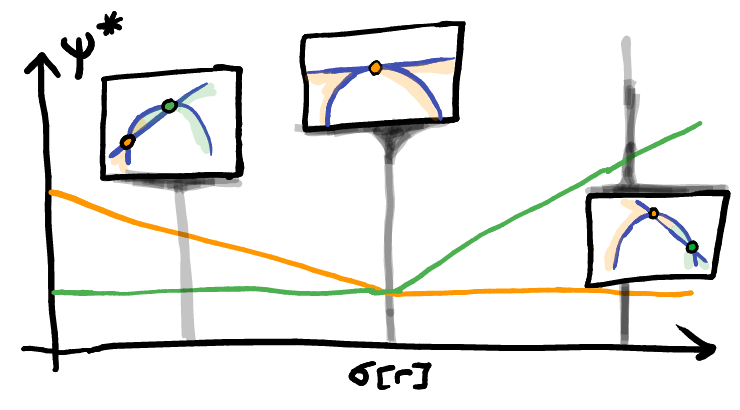
\includegraphics[scale=0.35]{figures/transcritical}
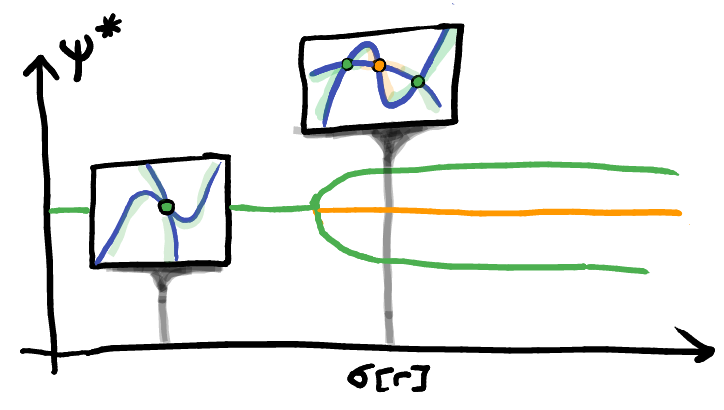
\includegraphics[scale=0.35]{figures/pitchfork}
\caption{Saddle-node, Transcritical and Pitchfork bifurcation diagram showing
\textcolor{Green}{stable} and \\\textcolor{orange}{unstable} fixed points $\psi^*$
as a function of parameter $\sigma[r]$. Insets show nullcline intersections.}
\label{fig:bifurcations}
\end{figure}
Another catagory of bifurcations involves limit cycles, which emerge from fixed
points where the linearised Jacobian eigenvalues have no real part. Limit cylces
have circulating field flow as shown in Figure \ref{fig:stability} along the
$\mathrm{Tr}[\mathbf{J}]=0$, $|\mathbf{J}|>0$ axis.

Note how oscillations emerge at small amplitudes in the Hopf bifurcation,
whereas the large amplitude oscillations may instantly emerge in an infinite-period
or cyclic-fold bifurcation. In Figure \ref{fig:limitcycles} the shaded regions
represent the peaks and troughs of the oscillations.
\begin{figure}[H]
\centering{}
\captionsetup{justification=centering}
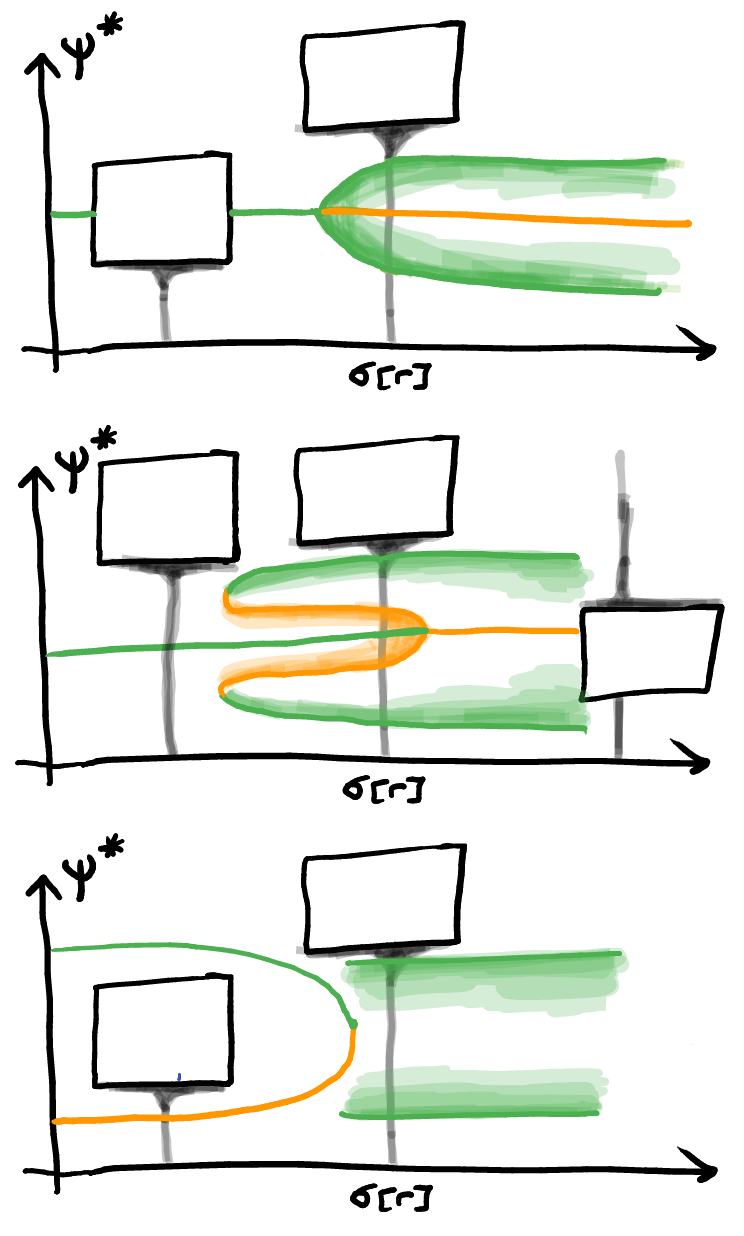
\includegraphics[scale=0.35]{figures/limitcycles}
\caption{Hopf, Cyclic-fold and Infinite-Period bifurcation diagram showing
\textcolor{Green}{stable} and \textcolor{orange}{unstable}\\ fixed points
and limit cycles as a function of parameter $\sigma[r]$.
Insets show nullclines [tbc]}
\label{fig:limitcycles}
\end{figure}
\subsubsection{Attractor Geometry and Universality}
In this section we would explore the geometrisation of phase space, lyapunov
exponents and universality. Perhaps a discussion on phase transitions and
the relation to Landau-Ginzberg approaches is required.
Maybe also periodic orbit theory? Depends how useful it is.
\subsubsection{Reaction-Diffusion}
Here we first introduce diffusion macroscopically by simply adding the laplacian
to mean field equation $\eqref{eq:reaction}$. We introduce the turning bifurcation and
show how linear stability analysis is insufficient to capture pattern formation
and rich inhomogenous steady states. A promising approach may be geometrisation
of the moving local equilibria \cite{Halatek2018}.

\pagebreak
\section{Field Theory Approach}\vspace{-10pt}
Taking the mean-field thermodynamic limit gives rise to a set of coupled nonlinear
ordinary differential equations, whos steady states and limit cylces can be investigated
readily. Timescales and dynamical information beyond linear stability however are more
difficult to extract. A field theory approach makes use of diagrammatic expansions
and Green's Functions allowing for calculation of correlations and observables.
\vspace{-15pt}
\subsection{Doi Representation}
\vspace{-10pt}
\subsubsection{Reaction Term}
\vspace{-10pt}
The starting point for setting up the field theory is casting of the nonlinear
equations of motion into a space in which the state evolves according to a linear
equation with the complexity compressed into the operator \cite{Doi1976}.

Suppose we define orthonormal basis $\ket{s}$ to represent $s[i]$ particles for
all species $i=1\dots S$. Discreteness suggests we should introduce field operators
$\hat{a}_i,\hat{a}_i^{\dagger}$ that remove/add one particle of species $i$ from/to the state
$\ket{s}$. Here $\delta_{ij}$ is the delta and the indicator vector $\mathbb{1}_i[j]:=\delta_{ij}$.
\begin{align}
	\begin{matrix}
		\hat{a}_i\ket{s}:=s[i]\ket{s-\mathbb{1}_i} &&& \hat{a}_i^{\dagger}\ket{s}:=\ket{s+\mathbb{1}_i}
	\end{matrix}
	\label{eq:fieldoperators}
\end{align}
It can be shown --- see Appendix \ref{a:doi} --- with such chosen
normalisation these operators
satisfy the usual bosonic commutation relations and define the number operator
in the usual way.
\begin{align}
	\begin{matrix}
		\hat{a}_i^{\dagger}\hat{a}_i\ket{s}=s[i]\ket{s}
	\end{matrix}
	\qquad\qquad
	\begin{matrix}
		[\hat{a}_i,\hat{a}_j^{\dagger}]=\delta_{ij} \\
		[\hat{a}_i,\hat{a}_j]=[\hat{a}_i^{\dagger},\hat{a}_j^{\dagger}]=0
	\end{matrix}
	\label{eq:commutationrelations}
\end{align}
Moreover it becomes possible to have an
operator representation of the propensity $\hat\omega(r)$ and shifts independent
of the state $s$.
\begin{align}
	\hat\omega(r)\ket{s}=\omega(r|s)\ket{s}
	\qquad
	\hat\omega(r):=
	\lambda[r]
	\prod_{i=1}^S
	\hat{a}_i^{\dagger g[i,r]}\hat{a}_i^{g[i,r]}
	\qquad
	\lambda[r]=
	\frac{\sigma[r]}{\prod_{i=1}^Sg[i,r]!}
	\label{eq:propensityoperator}
	\\
	\ket{s+n} =
	\prod_{i=1}^S\hat{a}_i^{\dagger n[i]}
	\ket{s}\qquad
	\text{where}\quad
	\hat{a}_i^{-\dagger}\ket{s}=\ket{s-\mathbb{1}_i}
	\qquad\qquad\qquad
	\label{eq:shiftoperator}
\end{align}
\pagebreak

Defining the time-dependent state $\ket{\Psi(t)}$ as a linear combination of all possible
states $\ket{s}$ with coefficients $\mathbb{P}(s,t)$ which evolve according to
the Chemical Master Equation \eqref{eq:cme} allows us to write down a Schr\"odinger
equation with Hamiltonian $\hat{\mathcal{R}}$. The equation can be obtained by using
the operator representation of the propensity and shifting indecies $s$ in the sum.
\begin{align}
	\mathbb{i}\,\partial_t\ket{\Psi(t)}
	=\hat{\mathcal{R}}\ket{\Psi(t)}
	\qquad\text{where}\quad
	\ket{\Psi(t)}:=\sum_{s\in\mathbb{N}^S}\mathbb{P}(s,t)\ket{s}
	\label{eq:reactionschrodinger}
\\
	\hat{\mathcal{R}} = \mathbb{i}\,
	\sum_{r=1}^R
		\lambda[r]
		\left(
			\prod_{i=1}^S\hat{a}_i^{\dagger\Gamma[i,r]}
			-
			\hat{\mathbb{1}}
		\right)
		\prod_{j=1}^S
			\hat{a}_j^{\dagger g[j,r]}
			\hat{a}_j^{g[j,r]}
	\qquad\qquad
	\label{eq:reactionhamiltonian}
\end{align}
Amazing! We are now ready to import methods from Quantum Mechanics from
diagrammatic expansions through to non-equilibrium Green's Functions and Feynman
path integrals. Let us pause and ponder this Hamiltonian: it is non-Hermitian
and therefore leads to irreversible dynamics; the term involving $g[i,r]$ is
zero unless the state contains $g[i,r]$ particles of species $i$, defining the
\textit{order} of reaction $r$; if the right species are present the term
involving $\Gamma[i,r]$ is non-zero for  $\Gamma[i,r]\neq 0$ with the state
change encoded by creation, and inverse-creation operators.
\vspace{-10pt}\subsubsection{Diffusion Term}\vspace{-10pt}
We consider diffusion on an $M$-dimensional lattice for a discrete state,
continous space-time process. For now lets consider a single species
$s\in\mathbb{N}$ and let $\mathbb{P}(s_{\mathbf{x}}\dots s_{\mathbf{y}},t)$ be
the joint probability of finding $s_{\mathbf{x}}\dots s_{\mathbf{y}}$ particles
in locations $\mathbf{x}\dots\mathbf{y}\in\mathbb{R}^M$ at time $t$. Particles
at $\mathbf{x}$ may jump to/from neightbrouhood $\partial\mathbf{x}$.
\begin{align}
	\partial_t \mathbb{P}(s_{\mathbf{x}}\dots s_{\mathbf{y}},t) &=
	D\int_{\mathbb{R}^{M}}\int_{\partial\mathbf{x}}\!
	(s_{\mathbf{y}}+1)\mathbb{P}(s_{\mathbf{x}}-1\dots s_{\mathbf{y}}+1,t)
	-
	s_{\mathbf{x}}\mathbb{P}(s_{\mathbf{x}}\dots s_{\mathbf{y}},t)
	\,\mathrm{d}\mathbf{y}\mathrm{d}\mathbf{x}
\end{align}
Intorducing orthonormal basis $\ket{s_{\mathbf{x}}\dots s_{\mathbf{y}}}$ and field
operators $\hat{a}(\mathbf{x})^{\dagger},\hat{a}(\mathbf{x})$ that add/remove particles
to/from location $\mathbf{x}$ as we did in Section 1.2.1 for the Chemical Master Equation,
allows us to represent diffusion as Hamiltonian $\hat{\mathcal{D}}$ acting on a linear
state space $\ket{\Psi(t)}$.
\begin{align}
	\mathbb{i}\,\partial_t\ket{\Psi(t)}
	=\hat{\mathcal{D}}\ket{\Psi(t)}
	\qquad\text{where}\quad
	\ket{\Psi(t)}:=\sum_{s_{\mathbf{x}}\dots s_{\mathbf{y}}\in\mathbb{N}}
	\mathbb{P}(s_{\mathbf{x}}\dots s_{\mathbf{y}},t)
	\ket{s_{\mathbf{x}}\dots s_{\mathbf{y}}}
	\label{eq:diffusionschrodinger}
\\
	\hat{\mathcal{D}} = -\frac{\mathbb{i}\,D}{2}
	\int_{\mathbb{R}^{M}}\int_{\partial\mathbf{x}}\!
		(\hat{a}(\mathbf{y})-\hat{a}(\mathbf{x}))^{\dagger}(\hat{a}(\mathbf{y})-\hat{a}(\mathbf{x}))
	\,\mathrm{d}\mathbf{y}\mathrm{d}\mathbf{x}
	\qquad\qquad\quad
	\label{eq:diffusionhamiltonian}
\end{align}
\pagebreak
\subsubsection{Reaction-Diffusion Hamiltonian}\vspace{-10pt}
Finally by extending the state space $\ket{s_\mathbf{x}\dots s_\mathbf{y}}$ to multiple particle
species $s_\mathbf{x}\in\mathbb{N}^S,\mathbf{x}\in\mathbb{R}^M$ we may bring together the contributions
from reaction and diffusion. In order to simplify results we can vectorise the field operators
$\hat{a}(\mathbf{x}),\hat{a}(\mathbf{x})^{\dagger}$ such that their $i$th components are the field
operators for particle species $i$. Note that $^{\dagger}$ acts on the operator and $^\top$ acts on the
vector, which may lead to inner or outer products.
\begin{align}
	\begin{matrix}
		\hat{a}(\mathbf{x})\ket{s_\mathbf{x}\dots s_\mathbf{y}}
		:=s_\mathbf{x}\ket{s_\mathbf{x}-1\dots s_\mathbf{y}} \\
		\hat{a}(\mathbf{x})^{\dagger}\ket{s_\mathbf{x}\dots s_\mathbf{y}}
		:=\ket{s_\mathbf{x}+1\dots s_\mathbf{y}} \\
		\hat{a}(\mathbf{x})^{\dagger}
		\hat{a}(\mathbf{x})
		\ket{s_\mathbf{x}\dots s_\mathbf{y}}=s_\mathbf{x}\ket{s_\mathbf{x}\dots s_\mathbf{y}}
	\end{matrix}
	\qquad\qquad
	\begin{matrix}
		[		\hat{a}(\mathbf{x}),
				\hat{a}(\mathbf{y})^{\dagger\top} ]=\mathbb{1}\delta(\mathbf{x}-\mathbf{y}) \\
				[		\hat{a}(\mathbf{x}),
						\hat{a}(\mathbf{y})^{\top} ]=		[		\hat{a}(\mathbf{x})^{\dagger},
										\hat{a}(\mathbf{y})^{\dagger\top} ]=\mathbb{0}
	\end{matrix}
	\label{eq:vectorfieldoperators}
\end{align}
The diffusion coefficients for each species are now the elements
of diagonal matrix $\mathbf{D}$ and reaction rates $\lambda(\gamma,\mathbf{x})$ may also acquire
spatial dependence. The state $\ket{\Psi(t)}$ now spans $\mathbb{N}^S\times\mathbb{R}^M$. We have
also rewritten the products of operators in the reaction term as exponentiated inner products
$\gamma^{\top}\!\ln \hat{a}(\mathbf{x})^{\dagger}=\sum_{i=1}^{S}\gamma[i]\ln\hat{a}_i(\mathbf{x})^{\dagger}$.
\begin{align}
	\mathbb{i}\,\partial_t\ket{\Psi(t)}
	=\int_{\mathbb{R}^M}\!\hat{\mathcal{H}}(\mathbf{x})\mathrm{d}\mathbf{x}\,
	\ket{\Psi(t)}
	\quad\text{where}\quad
	\ket{\Psi(t)}:=\sum_{s_{\mathbf{x}}\dots s_{\mathbf{y}}\in\mathbb{N}^S}
	\mathbb{P}(s_{\mathbf{x}}\dots s_{\mathbf{y}},t)
	\ket{s_{\mathbf{x}}\dots s_{\mathbf{y}}}
	\label{eq:schrodinger}
\\
	\hat{\mathcal{H}}(\mathbf{x}) =
	\mathbb{i}
	\sum_{\langle\gamma,g\rangle\in\mathbf{\Gamma}}
		\lambda(\gamma,\mathbf{x})
		\left(
			\mathbb{e}^{\,\gamma^{\top}\!\ln \hat{a}(\mathbf{x})^{\dagger}}
			-
			\hat{\mathbb{1}}
		\right)
			\mathbb{e}^{\,g^{\top}\!\left(\,
			\ln \hat{a}(\mathbf{x})^{\dagger}+\ln \hat{a}(\mathbf{x})
			\right)}
	\qquad\qquad\\
	-\frac{\mathbb{i}}{2}
	\int_{\partial\mathbf{x}}\,
		\left(\hat{a}(\mathbf{y})^{\dagger}-\hat{a}(\mathbf{x})^{\dagger}\right)^\top
		\!\mathbf{D}\,
		\big(\hat{a}(\mathbf{y})-\hat{a}(\mathbf{x})\big)
	\mathrm{d}\mathbf{y}
	\qquad\qquad\qquad\qquad
	\label{eq:hamiltonian}
\end{align}
\subsection{Green's Functions}\vspace{-10pt}
\subsubsection{Non-unitary Evolution Operator}\vspace{-10pt}
Solving \eqref{eq:schrodinger} formally suggests we define a non-unitary time independent
evolution operator $\hat{\mathcal{U}}(t,t')$. In the ordinary quantum cases this operator is unitary;
we will have to keep this in mind when applying the following methods.
\begin{equation}
\hat{\mathcal{U}}(t,t'):=
	\mathbb{e}^{-\mathbb{i}(t-t')\int\hat{\mathcal{H}}(\mathbf{x})\mathrm{d}\mathbf{x}}
	\qquad\qquad
	\begin{matrix}
		\hat{\mathcal{U}}(t,t')^\dagger\hat{\mathcal{U}}(t,t') \neq \mathbb{1}\\
		\hat{\mathcal{H}}(\mathbf{x})^\dagger \neq \hat{\mathcal{H}}(\mathbf{x})
	\end{matrix}
	\label{eq:evolutionoperator}
\end{equation}
\subsubsection{Dynamical Ensemble Averages}\vspace{-10pt}
Since the coefficients of state vector $\ket{\Psi(t)}$ directly yield probabilities,
$\mathbb{P}(s_{\mathbf{x}}\dots s_{\mathbf{y}},t)$ not probability amplitudes, ensemble
averages $\langle A(\mathbf{x},t)\rangle$ are calculated with a differently defined
density matrix $\hat\rho(t)$. One of the states in the outer product $\bra{\Psi(t)}$
is replaced by the unit projection state $\bra{\mathbb{p}}$. This state can be written
in terms of field operators; in fact it is the left eigenstate of the creation operator
--- a coherent state.
\begin{align}
	\left\langle A(\mathbf{x},t) \right\rangle=
	\text{Tr}\left[
	\,\hat\rho(t)\,\hat{\mathcal{A}}(\mathbf{x},t)
	\right]
	\quad\text{where}\quad\hat\rho(t):=\ket{\Psi(t)}\!\!\bra{\mathbb{p}}
	\label{eq:averages}
\end{align}
\vspace{-35pt}
\begin{align}
	\begin{matrix}
		\bra{\mathbb{p}}:=
		\sum_{s_{\mathbf{x}}\dots s_{\mathbf{y}}\in\mathbb{N}^S}
		\bra{s_{\mathbf{x}}\dots s_{\mathbf{y}}} \\
		=\bra{\varnothing}\mathbb{e}^{\int\mathrm{d}\hat a(\mathbf{x})}
		\qquad\qquad
	\end{matrix}
	\qquad\bra{\mathbb{p}}\hat{a}(\mathbf{x})^{\dagger}=\bra{\mathbb{p}}
	\label{eq:projectionoperator}
\end{align}
This modified definition of $\hat\rho(t)$ leads to a Liouville Equation and
Ehrenfest Theorem that do not involve commutators. Furthermore, the time
evolved density matrix no longer has $\hat{\mathcal{U}}(t,t')$ acting on
both sides.
\begin{align}\label{eq:liouville-ehrenfest}
\mathbb{i}\frac{\overrightarrow{d}}{dt}\hat\rho(t)=\hat{\mathcal{H}}\,\hat\rho(t)
\qquad\qquad
\mathbb{i}\frac{\overrightarrow{d}}{dt}\hat{\mathcal{A}}(\mathbf{x},t)
=\mathbb{i}
\,\partial_t\hat{\mathcal{A}}(\mathbf{x},t)
+\hat{\mathcal{A}}(\mathbf{x},t)\hat{\mathcal{H}}
\end{align}\vspace{-30pt}
\subsubsection{The Heisenberg Picture}\vspace{-10pt}
In the interacting picture the time dependance is shared between the observable
$\hat{\mathcal{A}}(\mathbf{x},t)$ and density $\hat\rho(t)$. Transforming out the
time dependance from the density into the operator using \eqref{eq:evolutionoperator}
brings the operator into the Heisenberg picture $\hat{\mathcal{A}}_H(\mathbf{x},t)$.
Letting the evolution $\,\hat{\mathcal{U}}(t):=\hat{\mathcal{U}}(t,0)$ and the
initial condition $\hat\rho:=\hat\rho(0)$ we can write
\begin{align}
	\left\langle A(\mathbf{x},t) \right\rangle=
	\text{Tr}\left[
	\,\hat\rho \,\hat{\mathcal{A}}_H(\mathbf{x},t)
	\right]
\qquad
\hat{\mathcal{A}}_H(\mathbf{x},t):=
\hat{\mathcal{A}}(\mathbf{x},t)\,\exp\left[{-\mathbb{i}\,t
\int_{\mathbb{R}^M}\!\hat{\mathcal{H}}(\mathbf{x})\,\mathrm{d}\mathbf{x}}
\right]
\label{eq:heisenbergpicture}
\end{align}
This allows an arbitrary choice for the density matrix, and focuses the dynamics
onto the operators. Commutators \eqref{eq:vectorfieldoperators} at equal times remain
the same, and time-independent operators like $\hat{a}(\mathbf{x})$ and
$\hat{a}(\mathbf{x})^{\dagger}$ pick up a time dependence from the evolution operator.
\subsubsection{Green's Functions \& the Hierarchy}
\vspace{-10pt}
Since both the Hamiltonian and any observable operator can be expressed in terms
of vector field operators $\hat{a}(\mathbf{x})$ and $\hat{a}(\mathbf{x})^{\dagger}$, all
dynamical ensemble averages \eqref{eq:heisenbergpicture} are are expressed in terms
of strings of field operators. It seems natural to attempt defining a building
block out of which one can express these averages. These objects are known as
Green's Functions and encode all correlations and responses of the system.
\begin{equation}\label{eq:green-function}
\mathbf{G}(\mathbf{x},t|\mathbf{y},t'):=
\frac{1}{\mathbb{i}}
\left\langle\mathcal{T}\left\{
\hat{a}(\mathbf{x},t)
\hat{a}(\mathbf{y},t')^{\dagger\top}
\right\}\right\rangle
\end{equation}
\vspace{-40pt}
\begin{align*}
\hat{a}(\mathbf{x},t)\text{ and } \hat{a}(\mathbf{y},t')^{\dagger}
\text{ are implicitly in the Heisenberg picture}\\
\mathcal{T}
\text{ is the time-ordering meta operator}\qquad\qquad\quad
\end{align*}
Above is what is known as a one-particle Green's Function. Substituting this
 into the Ehrenfest Theorem \eqref{eq:liouville-ehrenfest} leads to two-particle Green's Functions. This
is due to the nasty way in which the time derivative and time ordering meta-operator
interact. Repeated substitution of these objects reveals that $n$-particle
Green's Function is coupled to $n\pm1$ particle Green's Functions. This infinite set of coupled
differential equations is called the Martin-Schwinger Hierarchy \cite{stefanucci2013}. The time ordering operator $\mathcal{T}\{\,\,.\,\,\}$ is evaluated to obtain
explicit expressions for Green's Function in terms of greater/lesser and
retarded/advanced components. We drop the spatial dependance $\mathbf{x}$ to avoid
clutter.
\begin{equation}\label{eq:greater-lesser}
\overset{\text{Greater and Lesser Components}}
{\mathbf{G}(z,z')=
\theta(z,z')\mathbf{G}^{>}(z,z')+\theta(z',z)\mathbf{G}^{<}(z,z')}
\end{equation}
\begin{equation}\label{eq:retarded-advanced}
\overset{\text{Retarded / Advanced Components}}
{\mathbf{G}^{\pm}(t,t')=
\pm\theta\Big(\pm(t-t')\Big)\Big(\mathbf{G}^{>}(t,t')-\mathbf{G}^{<}(t,t')\Big)}
\end{equation}
\begin{equation}\label{eq:green-symmetry}
\overset{\text{Antisymmetry}}
{\mathbf{G}^{\gtrless}(t,t')^{\dagger}=-\mathbf{G}^{\gtrless}(t',t)}
\qquad
\overset{\text{Causality}}
{\mathbf{G}^{\pm}(t,t')^{\dagger}=\mathbf{G}^{\mp}(t',t)}
\end{equation}\vspace{-10pt}\\
Here $\theta(t-t')$ and $\theta(z,z')$ are
the Heaviside Step Functions which are nonzero for real $t>t'$ and complex
$z>z'$ time arguments respectively. These Green's Function possess useful symmetries: anti-symmetry inherited from fermion behaviour and another condition encoding causality. The use of Langreth Rules \cite{stefanucci2013} allows to conversion of contour integrals into real integrals.
\subsubsection{Noninteracting Equations of Motion}\vspace{-10pt}
Suppose the hamiltonian $\mathbf{h}(t)$ only has quadratic terms in
$\hat{a}(\mathbf{x}),\hat{a}(\mathbf{x})^\dagger$. This is effectively a
non-interacting case and decouples the one-particle equation
of motion from the hierarchy revealing that the Green's Function is the
wavefunction solution to the Schr\"odinger Equation with a dirac delta
excitation in the field. Presented are the  set of conjugate equations in
single particle orbital matrix form, where the derivative acts on the right and left
times respectively. Here $\mathbf I$ is the identity matrix.\vspace{-10pt}
\begin{equation}\label{eq:non-interacting}
\left[\mathbb{i}\frac{\overrightarrow{d}}{dt}-\mathbf{h}(t)\,\right]
\mathbf{G}(t,t')=\mathbf{e}(t,t')
\qquad
\mathbf{G}(t,t')
\left[-\mathbb{i}\frac{\overleftarrow{d}}{dt'}-\mathbf{h}(t')\,\right]
=\mathbf{e}(t,t')
\end{equation}\vspace{-15pt}
\begin{equation*}
\quad\text{where}\quad
\mathbf{e}(t,t')=\mathbf{I}\,\delta(t,t')
\quad
[\,\mathbf h(t)\,]_{i,j}=\bra{i}\hat h(t)\ket{j}
\end{equation*}
\subsubsection{The Dyson Equation}\vspace{-10pt}
Using complex convolutions on the Keldysh Contour $\gamma$, inverses and
group properties that the Green's Functions obey, its possible to get rid of the time derivative in the equations of motion \eqref{eq:non-interacting} and derive the Dyson Equation.
This formula expresses the coupled Green's Function $\mathbf{G}(t,t')$ in terms of the isolated Green's Function $\mathbf{g}(t,t')$  , which is obtained by considering the diagonal elements of $\mathbf{h}(t)$ only.
These are convoluted with the self-energy $\mathbf\Sigma(t,t')$, which can not always be expressed explicitly, but still obeys the same symmetry properties \eqref{eq:green-symmetry} as the Green's Functions. The convolution variables match up in the same way matrix multiplication
indexes do.\vspace{-10pt}
\begin{equation}\label{eq:dyson}
\mathbf{G}_{}(t,t')=
\mathbf{g}(t,t')+\mathbf{g}\circ
\mathbf{\Sigma}\circ\mathbf{G}(t,t')=
\mathbf{g}(t,t')+\mathbf{G}\circ
\mathbf{\Sigma}\circ\mathbf{g}(t,t')
\end{equation}
\begin{equation*}
\quad\text{where}\quad
\mathbf a\circ\mathbf b\;(t,t')=
\int_\gamma\!\mathbf a(t,\tau)\mathbf b(\tau,t')\,\mathrm{d}\tau
\qquad
\mathbf{\Sigma}(t,t')
\text{ is the self-energy}
\end{equation*}
\subsubsection{The Keldysh Equation}\vspace{-10pt}
The analogue of the Dyson equation, projected into  greater/lesser
and retarded/advanced  subspace, done readily with the help of Langreth Rules, is known as the Keldysh Equation.
This equation is used to investigate the steady state behaviour.
\vspace{6pt}
\begin{align}\label{eq:keldysh}
\mathbf{G}^{\gtrless}(t,t')=
\overset{\text{Transient Term}}
{\left(
\mathbf{e}+\mathbf{G}^{+}\bullet\mathbf{\Sigma}^{+}
\right)
\bullet\mathbf{g}^{\gtrless}\bullet
\left(
\mathbf{e}+\mathbf{\Sigma}^{-}\bullet\mathbf{G}^{-}
\right)(t,t')}+
\overset{\text{Steady State Term}}
{\mathbf{G}^{+}
\bullet\mathbf{\Sigma}^{\gtrless}\bullet
\mathbf{G}^{-}(t,t')}
\end{align}
\vspace{-22pt}
\begin{equation*}
\quad\text{where}\quad
\mathbf a\bullet\mathbf b\;(t,t')=
\int_{t_0}^{\infty}\!\mathbf{a}(t,\tau)\mathbf{b}(\tau,t')\,\mathrm{d}\tau
\end{equation*}
\subsubsection{Time Independent Steady State Regime}\label{s2.3.5}
The Hamiltonian is time independent
$\mathbf h(t)=\mathbf h$ if all external influences are also time independent.
This makes all Green's  Functions components $\mathbf G^{\mathrm X}(t,t')$ -
among which are the advanced/retarded and greater/lesser components - depend
on real time differences $\tau=t-t'$, and the time translation invariance  allows
their representations in fourier space.
\begin{equation}\label{eq:fourier-representation}
\overset{\text{Component Fourier Transforms}}
{\mathbf{G}^{\mathrm X}(\omega)=
\int_{-\infty}^{\infty}\!\mathbf{G}^{\mathrm X}(\tau)
e^{\mathbb i\omega\tau}\,\mathrm{d}\tau
\qquad
\mathbf{G}^{\mathrm X}(t,t')=
\frac{1}{2\pi}\int_{-\infty}^{\infty}\!\mathbf{G}^{\mathrm X}(\omega)
e^{-\mathbb i\omega(t-t')}\,\mathrm{d}\omega}
\end{equation}
\vspace{-10pt}\\
Note that
 convolution $\bullet$ as defined in equation \eqref{eq:keldysh} reduces to regular fourier convolution
if $t_0=-\infty$ ; this puts the dynamics far from initial conditions, in the steady state regime. According to the convolution theorem,  applying the fourier transform $\mathcal{F}[\;.\;]$ to convolutions of two functions retrieves the product of their  individual fourier transforms. The Keldysh Equation \eqref{eq:keldysh} yields another powerful simplification.
\vspace{7pt}
\begin{equation}\label{eq:steady-state-symmetry}
\overset{\text{Time Independent Relations}}
{\mathbf{G}^{+}(\omega)-\mathbf{G}^{-}(\omega)=
\mathbf{G}^{>}(\omega)-\mathbf{G}^{<}(\omega)}
\end{equation}
\begin{equation*}
\overset{\text{Steady State Convolution }
\qquad\qquad\qquad\qquad
\text{Steady State Keldysh Equation}}{}
\end{equation*}\vspace{-35pt}
\begin{equation*}
\mathcal{F}[\,\mathbf{a}\bullet\mathbf{b}\;(t,t')]=
\mathbf{A}(\omega)\mathbf{B}(\omega)
\qquad\Rightarrow\qquad
\mathbf{G}^{\gtrless}(\omega)=
\mathbf{G}^{+}
(\omega)\mathbf{\Sigma}^{\gtrless}(\omega)
\mathbf{G}^{-}(\omega)
\end{equation*}

\pagebreak
\section{Model Systems}\vspace{-10pt}
\subsection{Lotka--Volterra}\vspace{-10pt}
The Lotka--Volterra model is a canonical example of a predator-prey dynamical
system. Here we may summarise the reactive behaviour between predators $A(t)$
and prey $B(t)$ in Feynman diagrams. Particles are represented by arrows
$\rightarrow$ and reactions by wavy arrows $\leadsto$.
\begin{figure}[H]
\centering{}
\captionsetup{justification=centering}
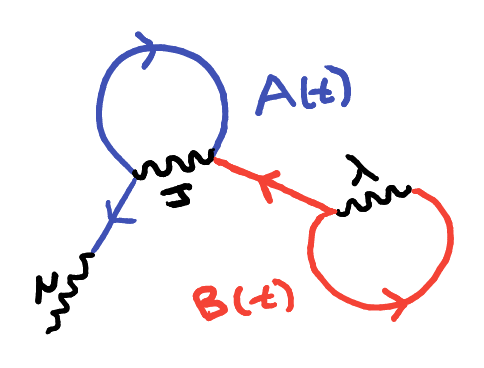
\includegraphics[scale=0.4]{figures/lotkavolterrafield}
\caption{Feynman diagram of the Lotka--Volterra field ${A\choose B\,}$  revealing
autocatalytic birth \\ rate $\lambda$ for prey, constant death rate $\mu$ for predators
and predator--prey interaction $J$}
\label{fig:lotkavolterrafield}
\end{figure}
Letting $s(t)={A\choose B\,}$, the stoichiometric matrix $\mathbf{\Gamma}$ and
propensity $\omega(s|\mathbf{\Gamma})$ are determined from the state changes
$\gamma$ and the rates of each reaction $\sigma(\gamma)=\mu,\lambda,J$. It
can easily be seen that the mean field approximation \eqref{eq:reaction}
now yields the well-known equations.
\begin{align}
	\mathbf{\Gamma}=
	\begin{pmatrix}
		-1 & 0 & 1 \\
		0 & 1 & -1 \\
	\end{pmatrix}
	\qquad\qquad
	\omega(s|\mathbf{\Gamma})=
	\begin{pmatrix}
	  \mu A(t)\\
		\lambda B(t)  \\
		J A(t)B(t) \\
	\end{pmatrix}
\end{align}
Figure \ref{fig:lotkavolterraspace} reveals that this reaction topology produces
nullcines that intersect to form a stable limit cycle. The amplitude is governed
by the initial conditions and time period by the death and birth rates. According
to the reaction term \eqref{eq:reactionhamiltonian} the Hamiltonian for predator
field $\hat a$ and prey field $\hat b$ is
\begin{equation}
	\mathcal{R}=\mathbb{i}
	\left(
		\mu (1-\hat a^\dagger)\hat a
		+ \lambda (\hat b^{\dagger2}-\hat b^\dagger)\hat b
		+ J (\hat a^{\dagger2}-\hat a^\dagger \hat b^\dagger) \hat a \hat b
	\right)
\end{equation}
\begin{figure}[H]
\centering{}
\captionsetup{justification=centering}
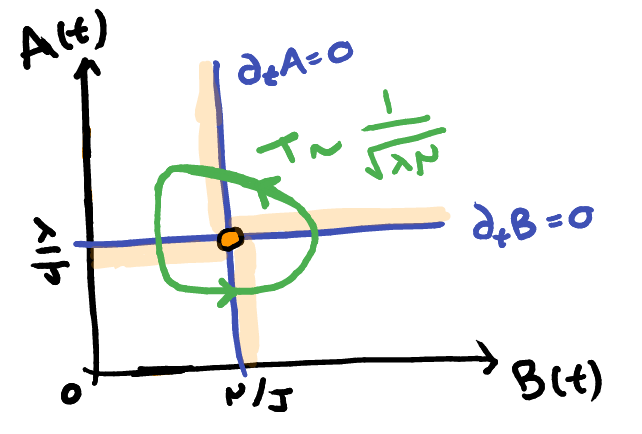
\includegraphics[scale=0.4]{figures/lotkavolterraspace}
\caption{Predator--prey field nullcines intersecting at unstable
fixed point\\ giving rise to stable limit cycle
whos time period $T\sim 1/\sqrt{\lambda\mu}$ }
\label{fig:lotkavolterraspace}
\end{figure}

\subsection{Michaelis--Menten}
\begin{figure}[H]
\centering{}
\captionsetup{justification=centering}
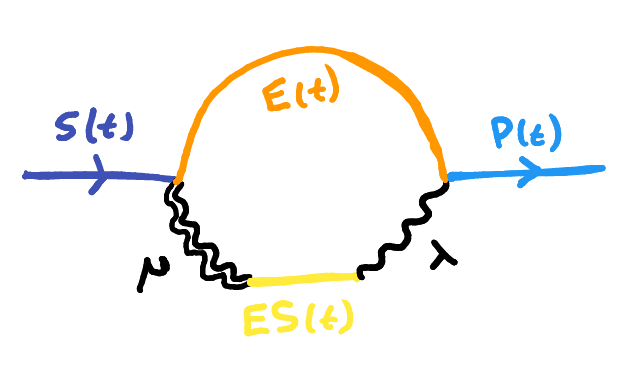
\includegraphics[scale=0.35]{figures/michaelismentenfield}
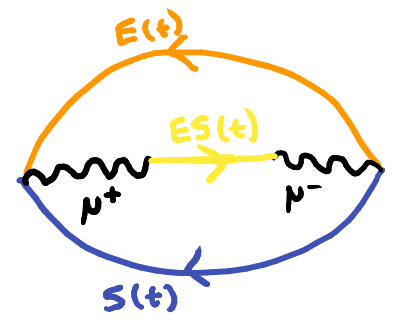
\includegraphics[scale=0.35]{figures/reversiblefield}
\caption{Feynman diagram of the Michaelis--Menten field $(S,E,ES,P)$ showing \\
reversible substrate--enzyme reaction $\mu$ and irreversible complex to product
reaction $\lambda$}
\label{fig:michaelismentenfield}
\end{figure}
\bibliography{mendeley_v2}
\bibliographystyle{ieeetr}

\appendix
\section{Chemical Master Equation}\label{a:cme}
The Chemical Master Equation a specific case of the differential form of the
Chapman-Kolmogorov equation, which in turn is a consequence of the Markov property and
considering transitions rates at infinitesimal time intervals. Starting with
the law of total probability
\begin{align}
	\mathbb{P}(s,t+\mathrm{d}t) &=
	\sum_{s'} \mathbb{P}(s,t+\mathrm{d}t|s',t)\mathbb{P}(s',t)
\end{align}
and probability of state change in a small interval $\mathrm{d}t$
\begin{align}
	\mathbb{P}(s,t+\mathrm{d}t|s',t)=
		\delta(s-s')\left(1-\sum_{r=1}^R \omega(r|s')\mathrm{d}t\right)
		+\sum_{r=1}^R \delta(s-s'-\mathbf{\Gamma}[r])\omega(r|s')\mathrm{d}t
\end{align}
where the first term is the probability of no reaction occuring, and the
second term restricts the possible state changes to those given by
the stoichiometric matrix $\mathbf{\Gamma}$. Upon substitution into
the total law of probability the Kronecker deltas $\delta$ filter the sum
over $s'$ leaving
\begin{align*}
	\mathbb{P}(s,t+\mathrm{d}t)-\mathbb{P}(s,t) &=
	\sum_{r=1}^R  \omega(r|s-\mathbf{\Gamma}[r])\mathrm{d}t\,\mathbb{P}(s-\mathbf{\Gamma}[r],t)-
	\omega(r|s)\mathrm{d}t\,\mathbb{P}(s,t)
\end{align*}
Dividing by $\mathrm{d}t$ and indentifying the time derivative
on the left hand side recovers \eqref{eq:cme}. Now to get the
equation for the first moment $\langle s \rangle$ we multiply by
$s$ and sum over sets $\mathbb{N}^S$
\begin{align*}
	\sum_{s\in\mathbb{N}^S}\partial_t\mathbb{P}(s,t) s &=
	\sum_{s\in\mathbb{N}^S}\sum_{r=1}^R
	\omega(r|s-\mathbf{\Gamma}[r])\mathbb{P}(s-\mathbf{\Gamma}[r],t)s-\omega(r|s)\mathbb{P}(s,t)s\\
	\partial_t\sum_{s\in\mathbb{N}^S}\mathbb{P}(s,t) s &=
	\sum_{r=1}^R \sum_{s\in\mathbb{N}^S}
	\omega(r|s)\mathbb{P}(s,t)(s+\mathbf{\Gamma}[r])-\omega(r|s)\mathbb{P}(s,t)s\\
	\partial_t\langle s \rangle &=
	\sum_{r=1}^R
	\mathbf{\Gamma}[r]
 \left\langle\,
	\omega(r|s)
	\,\right\rangle
\end{align*}
Recognising the matrix-vector multiplication with the stoichiometric matrix
prompts us to vectorise the propensity $\omega(s|\mathbf{\Gamma})\in[0,\infty)^R$.
The nonlinear propensity couples to higher order moments, unfolding the
heirarchy \eqref{eq:momentheirarchy}.

\section{Doi Representation}\label{a:doi}
Using the defining action of the field operators \eqref{eq:fieldoperators} it is
possible to verify the bosonic commutation relations, the operator
representation of propensity and shifts in state space.
\subsection{Commutation Relations}
\begin{align*}
		(\hat{a}_i \hat{a}_j^{\dagger}-\hat{a}_j^{\dagger}\hat{a}_i)
		\ket{s}&=(s[i]+\delta_{ij}-s[i])\ket{s+\mathbb{1}_j-\mathbb{1}_i}\\
		&=\delta_{ij}\ket{s+\mathbb{1}_j-\mathbb{1}_i}
\end{align*}
\vspace{-30pt}
\begin{align*}
		(\hat{a}_i^{\dagger}\hat{a}_j^{\dagger}-\hat{a}_j^{\dagger}\hat{a}_i^{\dagger})
		\ket{s}&=(1-1)\ket{s+\mathbb{1}_j+\mathbb{1}_i}
	\\ &=0
\end{align*}
\vspace{-30pt}
\begin{align*}
		(\hat{a}_i\hat{a}_j-\hat{a}_j\hat{a}_i)
		\ket{s}&=((s[i]-\delta_{ij})s[j]-(s[j]-\delta_{ij})s[i])\ket{s-\mathbb{1}_j-\mathbb{1}_i}
		\\
		&=\delta_{ij}(s[i]-s[j])\ket{s-\mathbb{1}_j-\mathbb{1}_i}\\
		&=0
\end{align*}
\subsection{Propensity}
Note that repeated application of the annihilation operator brings
out combinatorial factors, and subsequent application of the
creation operator can bring back the ket to its original state without
further factors coming out
\begin{align*}
		\hat{a}_i^n\ket{s}
		&=(s[i]-n+1)\dots(s[i]-1)s[i]\ket{s-n\mathbb{1}_i}\\
		&=\frac{s[i]!}{(s[i]-n)!}\ket{s-n\mathbb{1}_i}\\
		&=n!{s[i] \choose n}\ket{s-n\mathbb{1}_i}
\end{align*}
\vspace{-30pt}
\begin{align}
		\implies\qquad\frac{1}{n!}\hat{a}_i^{\dagger n}\hat{a}_i^n\ket{s}
		&={s[i] \choose n}\ket{s}\qquad\qquad\qquad
\end{align}
Knowing the eigenstate operator representation of the combinatoric
factor involving $s[i]$ and letting $\hat{\omega}(r)\ket{s}=\omega(r|s)\ket{s}$,
we can see from the general form of the propensity
\eqref{eq:propensity} that
\begin{align*}
	\hat\omega(r)=
	\sigma[r]
		\prod_{i=1}^S
		\frac{\hat{a}_i^{\dagger g[i,r]}\hat{a}_i^{g[i,r]}}{g[i,r]!}
\end{align*}
We note that the products of $g[i,r]!$ simply renormalise the reaction rate
$\sigma[r]$ suggesting we define renormalised propensity $\lambda[r]$ recovering
equations \eqref{eq:propensityoperator}. We also note that it is possible to
express the product over species $i$ in a compact form as a normal ordered inner
product
\begin{align}
	\hat\omega(r)=
	\lambda[r]\,
		\mathbb{e}^{\,g(r)^{\top}\left(\,\ln\hat{a}^{\dagger}+\ln\hat{a} \,\right)}
		\qquad\qquad\quad\\
		\text{where}\qquad
		\hat{a}=(\hat{a}_1\dots \hat{a}_S)\quad
		g(r)=(g[1,r]\dots g[S,r])
\end{align}
\subsection{Shifts}
\vspace{-10pt}
Noting that while there exists no inverse of the annihilation operator --- since
it is not possible to account for the case when $s[i]=0$ --- the creation
operator has a simple inverse
\begin{align*}
	\hat{a}_i^{-\dagger}\hat{a}_i^{\dagger}\ket{s}
	& :=\ket{s}\\
	&=\hat{a}_i^{-\dagger}\ket{s+\mathbb{1}_i}
	\qquad\implies\qquad
	\hat{a}_i^{-\dagger}\ket{s}
	=\ket{s-\mathbb{1}_i}
\end{align*}
and hence \eqref{eq:shiftoperator} is easily verified.
\subsection{Reaction Term}
Suppose we define a state vector spanning the space of all possible states
$s\in\mathbb{N}^S$. Inspired by quantum mechanics, we let the coefficients
of this vector be probability $\mathbb{P}(s,t)$ as given by definition
\eqref{eq:reactionschrodinger} and derive its equation of motion
\begin{align*}
	\partial_t\ket{\Psi(t)}
	&=\sum_{s\in\mathbb{N}^S}\partial_t\mathbb{P}(s,t)\ket{s}
	\\
	&=\sum_{s\in\mathbb{N}^S}\sum_{r=1}^R
	\omega(r|s-\mathbf{\Gamma}[r])\mathbb{P}(s-\mathbf{\Gamma}[r],t)\ket{s}
	-\omega(r|s)\mathbb{P}(s,t)\ket{s}
	\\
	&=\sum_{r=1}^R
	\sum_{s\in\mathbb{N}^S}\omega(r|s)\mathbb{P}(s,t)\ket{s+\mathbf{\Gamma}[r]}
	-\hat{\omega}(r)\sum_{s\in\mathbb{N}^S}\mathbb{P}(s,t)\ket{s}
	\\
	&=\sum_{r=1}^R
	\prod_{i=1}^S
	\hat{a}_i^{\dagger\Gamma[i,r]}
	\sum_{s\in\mathbb{N}^S}
	\omega(r|s)\mathbb{P}(s,t)\ket{s}
	-\hat{\omega}(r)\sum_{s\in\mathbb{N}^S}\mathbb{P}(s,t)\ket{s}
	\\
	&=\sum_{r=1}^R
	\left(
	\prod_{i=1}^S
	\hat{a}_i^{\dagger\Gamma[i,r]}
	-\hat{\mathbb{1}}
	\right)
	\hat{\omega}(r)\sum_{s\in\mathbb{N}^S}
	\mathbb{P}(s,t)\ket{s}
\end{align*}
Indentifying the state vector $\ket{\Psi(t)}$ on the right-hand-side
and multiplying by the imaginary factor $\mathbb{i}$ recovers the Hamiltonian
\eqref{eq:reactionhamiltonian}.
\end{document}
